\documentclass{article}
\usepackage[margin=1.0in]{geometry}
\usepackage[usenames, dvipsnames]{color}
\usepackage{longtable}
\usepackage[flushleft]{threeparttable}
\usepackage[justification=centering]{caption}
\usepackage{tikz}
\usepackage{pgfplots}
\usepackage{amsthm}
\usepackage{amsmath}
\usepackage{amssymb}
\usepackage[sc]{mathpazo}
\usepackage{microtype}
\usepackage[english]{babel}
\usepackage{titlesec}
\usepackage{physics}
\usepackage{float}
\usepackage{fancybox,framed}
\usepackage{graphicx}
\usepackage{caption}
\usepackage{subcaption}
\usepackage{cprotect}
\titleformat{\section}[block]{\large\scshape}{\thesection.}{1em}{} 
\titleformat{\subsection}[block]{\large}{\thesubsection.}{1em}{}

\newcommand\tab[1][1cm]{\hspace*{#1}}
\renewcommand\op[1]{\hat{#1}}
\title{PHYS 512 - Assignment 2}
\author{André Vallières (260742187)}
\date{\today}

\begin{document}
\maketitle

\section*{Problem 1}
For this problem, I have thought of two ways of saving processing time by reducing the number of calls to $f(x)$:
\begin{itemize}
    \item[1)] Reuse values computed for boundary values
    \item[2)] Build and use a cache as calculations are executed
\end{itemize}

The big advantage of the first method is that it comes with almost no memory cost and can easily save precious computing time. However, it does not guarantee that $f(x)$ won't be computed more than once for the same $x$. On the other hand, the second method does guarantee this by building and using a mapping $x \rightarrow f(x)$ for each value of $x$. This, however, comes with a memory cost, but is only of the order of kilobytes even for a tolerance of $10^{-11}$. Since insertion and access for a hashmap is of the order of $\mathcal{O}(1)$, the cache itself does not add any computing overhead. 

Fig. 1 compares these two methods with the simple bare method for a set of tolerances. As expected, method 2 requires less function calls than method 1, which itself requires less function calls than the bare method. In the case of Fig. 1b, method 2 requires, on average, 300 function calls less than the bare method, and method 1 requires, on average, 600 function calls less than method 1. 

\begin{figure}[h!]
\centering
\begin{subfigure}{.5\textwidth}
  \centering
  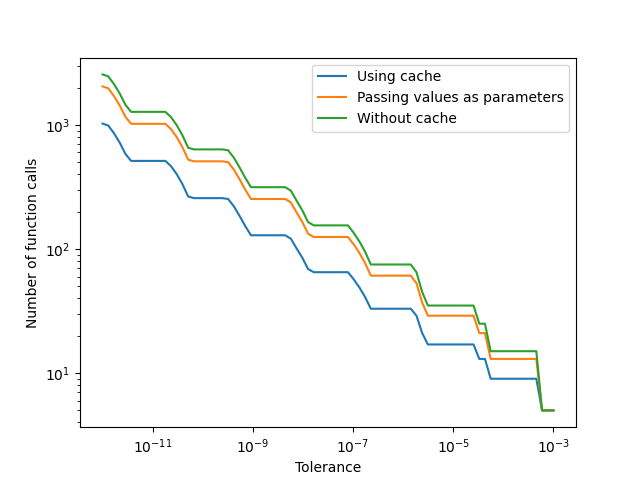
\includegraphics[width=\linewidth]{images/prob1_exp.png}
  \caption{}
\end{subfigure}%
\begin{subfigure}{.5\textwidth}
  \centering
  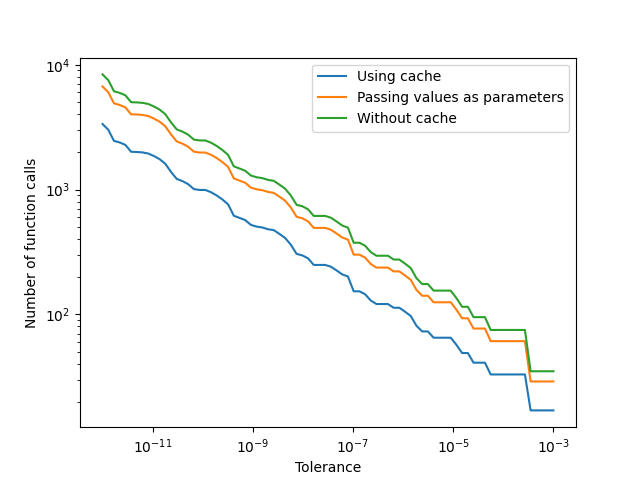
\includegraphics[width=\linewidth]{images/prob1_lorentzian.png}
  \caption{}
\end{subfigure}
\caption{Number of function calls required for integration at various tolerances, comparing the bare method with two optimization methods. (a) Integration of $e^x$ in the range $[0, 1]$. (b) Integration of $1/(1 + x^2)$ in the range $[-1, 1]$.}
\label{fig:prob1}
\end{figure}
\newpage

\section*{Problem 2}
To model $\log_2(x)$ in the range $[0.5, 1]$, we build the Chebyshev matrix and uses truncated versions of it to find what's the minimum order for which the accuracy is less than $10^{-6}$. Doing so yields the results shown in Fig. 2.
\begin{figure}[h]
    \centering
    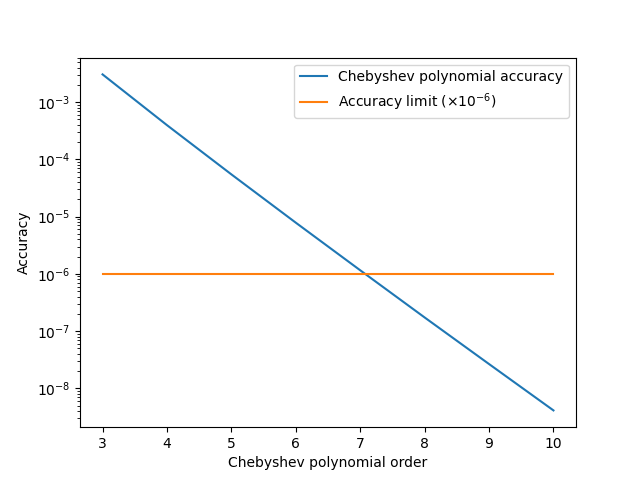
\includegraphics[scale=0.55]{images/prob2_cheb_acc.png}
    \caption{Chebyshev fit accuracy for various polynomial orders. Note that the lowest order for which the accuracy is less than $10^{-6}$ is 8. The accuracy for order 7 is around $1.15 \times 10^{-6}$.}
\end{figure}

Note that to make use of the full range for which Chebyshev polynomials have their useful properties, we compute $y=f(x)$ for $x \in [0.5, 1]$, but then rescale the $x$ array so that it is in the range $[-1, 1]$. With these results, we find that the lowest order for which the accuracy is less than $10^{-6}$ is 8. Equipped with this information, we may now perform Legendre polynomial fitting using the same points and order then compare the results.

Fig. 3 shows the residuals for Chebyshev and Legendre polynomials. The RMS errors are $1.94 \times 10^{-7}$ for Chebyshev and $1.84 \times 10^{-7}$ for Legendre. The maximum errors are $3.2 \times 10^{-7}$ for Chebyshev and $8.1 \times 10^{-7}$ for Legendre. Notice that Chebyshev has higher RMS error while Legendre has larger maximum error.
\begin{figure}[h]
    \centering
    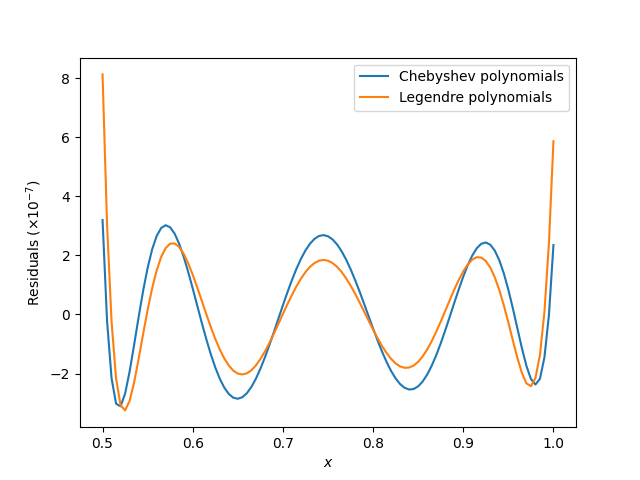
\includegraphics[scale=0.55]{images/prob2_residuals.png}
    \caption{Residuals for fitting $\log_2(x)$ in the range $[0.5, 1]$ using Chebyshev and Legendre polynomials.}
\end{figure}

\newpage
\section*{Problem 3}
\begin{itemize}
    \item[a)] The problem is set up by writing a system of 15 differential equations, each representing the time evolution of a decay product (or U-238). Since the half-lives differ greatly, we opted for the implicit Runge-Kutta method (i.e., \verb|Radau| in scipy) which should be able to handle stiff equations better. The results are shown in Fig. 4.

    \begin{figure}[h]
        \centering
        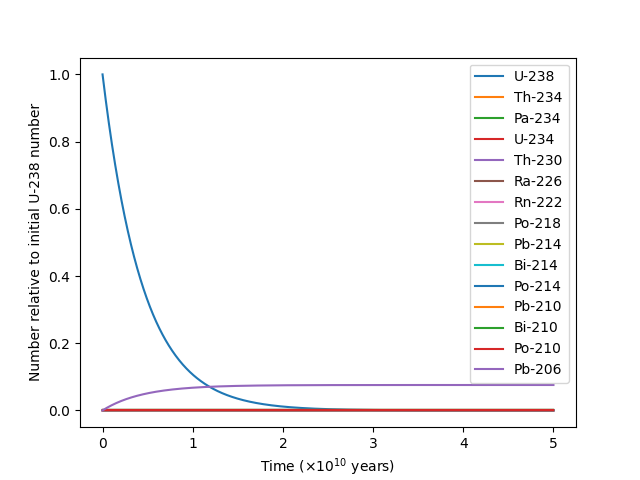
\includegraphics[scale=0.56]{images/prob3_u238_decay.png}
        \caption{U-238 decay plot showing all products of the decay chain assuming starting from a sample of pure U-238.}
    \end{figure}
    
    \item[b)] Plots of the ratio of Pb-206 to U-238 and Th-230 to U-234 are shown in Fig. 5. The results do make sense analytically. For Fig. 5a, we can approximate U-238 decaying directly into Pb-206 with an effective half-time, which would result in an exponentially increasing amount of Pb-206, as shown in the figure. For Fig. 5b, since Th-230 comes directly after U-234 in the decay chain, we also expected an increasing exponential behavior, but notice how the rate is decreasing since the half-life of Th-230 is smaller than U-234. Not shown in this plot is that eventually everything will decay into the final product, Pb-206.
    \begin{figure}[h!]
    \centering
    \begin{subfigure}{.5\textwidth}
      \centering
      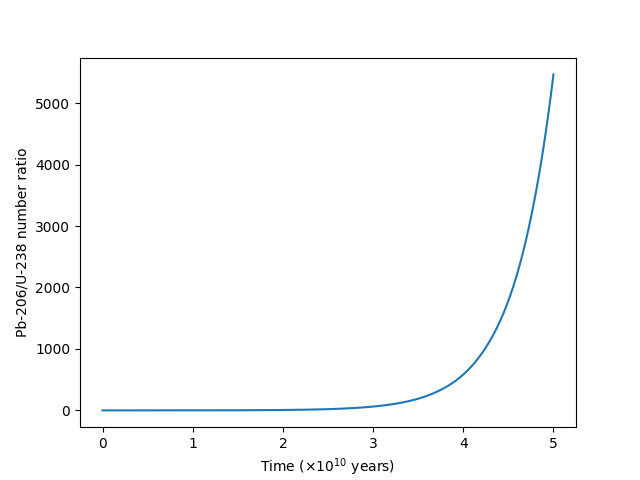
\includegraphics[width=\linewidth]{images/prob3_pb206_u238.png}
      \caption{}
    \end{subfigure}%
    \begin{subfigure}{.5\textwidth}
      \centering
      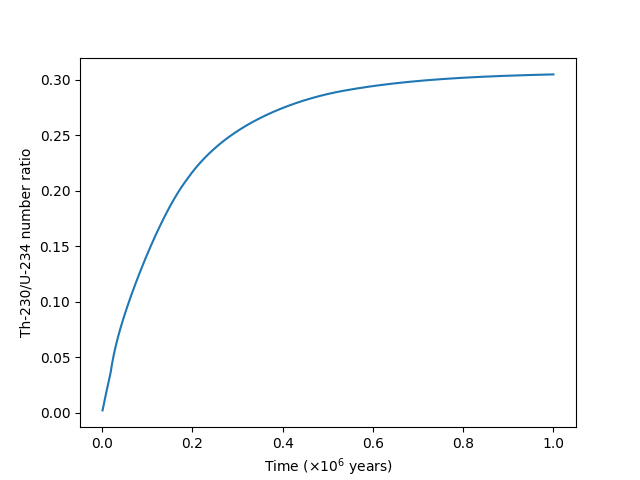
\includegraphics[width=\linewidth]{images/prob3_th230_u234.png}
      \caption{}
    \end{subfigure}
    \caption{Ratios of decay products over time. (a) Ratio of Pb-206 to U-238, the end product and initial sample, respectively. (b) Ratio of Th-230 to U-234, two consecutive decay products.}
    \label{fig:prob1}
    \end{figure}
    
\end{itemize}

\end{document}